\documentclass{article}

\usepackage{graphicx}
\usepackage[utf8]{inputenc}

\title{Exabiome Journal}
\author{kellyhuang }
\date{August 2020}

\begin{document}

\maketitle

\section{Multi-Head Self-Attention Experiments}

Multi-Head Self-attention was used after the convolution layers and before the linear layers of Roznet. These experiments were trained with the following parameters: 

-M -g 4 -b 32 -s 3001 -S 1000 -W 1000 --lr 0.0001

(Note: We used a lower learning rate which have contributed to the improvement of the accuracy scores and validation loss)

Using 4 self-attention heads produced the best results as there was continuous and significant improvement after each run. As the number of self-attention heads increased, there was more fluctuation between each run. 32 self-attention heads produced an out of memory error so the maximum number of attention heads that can be used with Roznet is 16. 


\subsection*{Medium dataset: 4 heads - 80 epochs per run}
Every run improved the accuracy of the model, compared to Roznet and Roznet with self-attention which began to converge at an accuracy scores of ~75\% and ~77\%. Each 4 hour run reached the maximum time limit at 80 epochs. The best results were achieved on the 304/320 epoch, with an accuracy of 82.04\% which is about ~5\% higher than Roznet with self-attention. With more runs, this model will continue to improve. 

Also note that this model is distinguishing between the red and orange blob which was stacked on top of each other in previous models. Though there is improvement, the green blob underneath is still not as distinguishable. 

\begin{figure}[h!]
  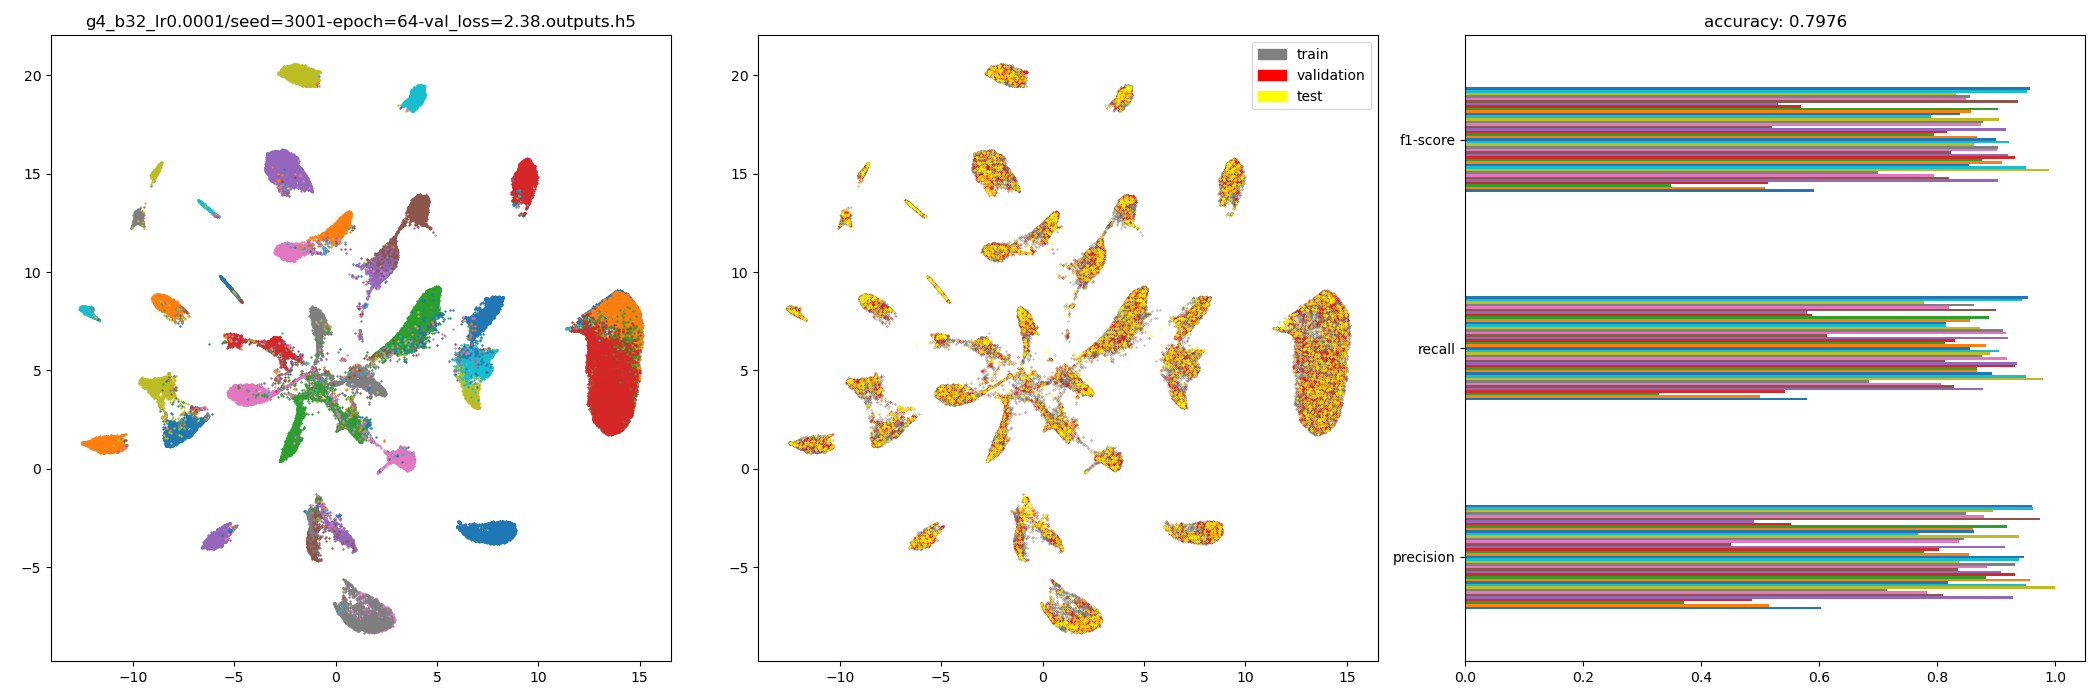
\includegraphics[width=\linewidth]{new_journal/figures/experiments/roznet_multi/4_heads/run1.png}
  \caption{Run 1}
\end{figure}

\begin{figure}[h!]
  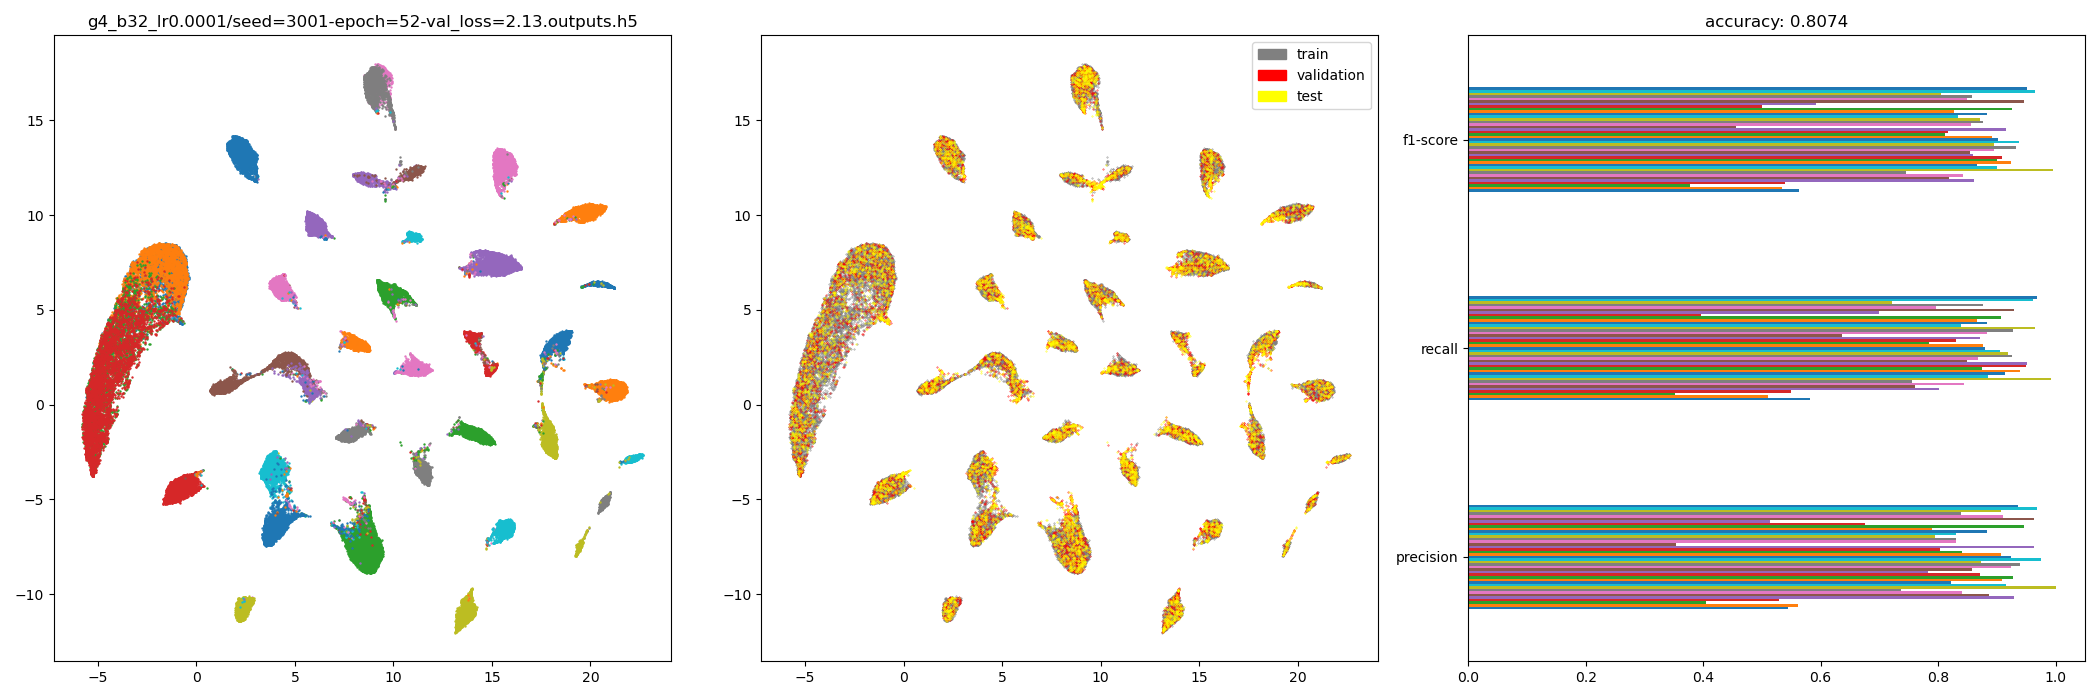
\includegraphics[width=\linewidth]{new_journal/figures/experiments/roznet_multi/4_heads/run2.png}
  \caption{Run 2}
\end{figure}

\begin{figure}[h!]
  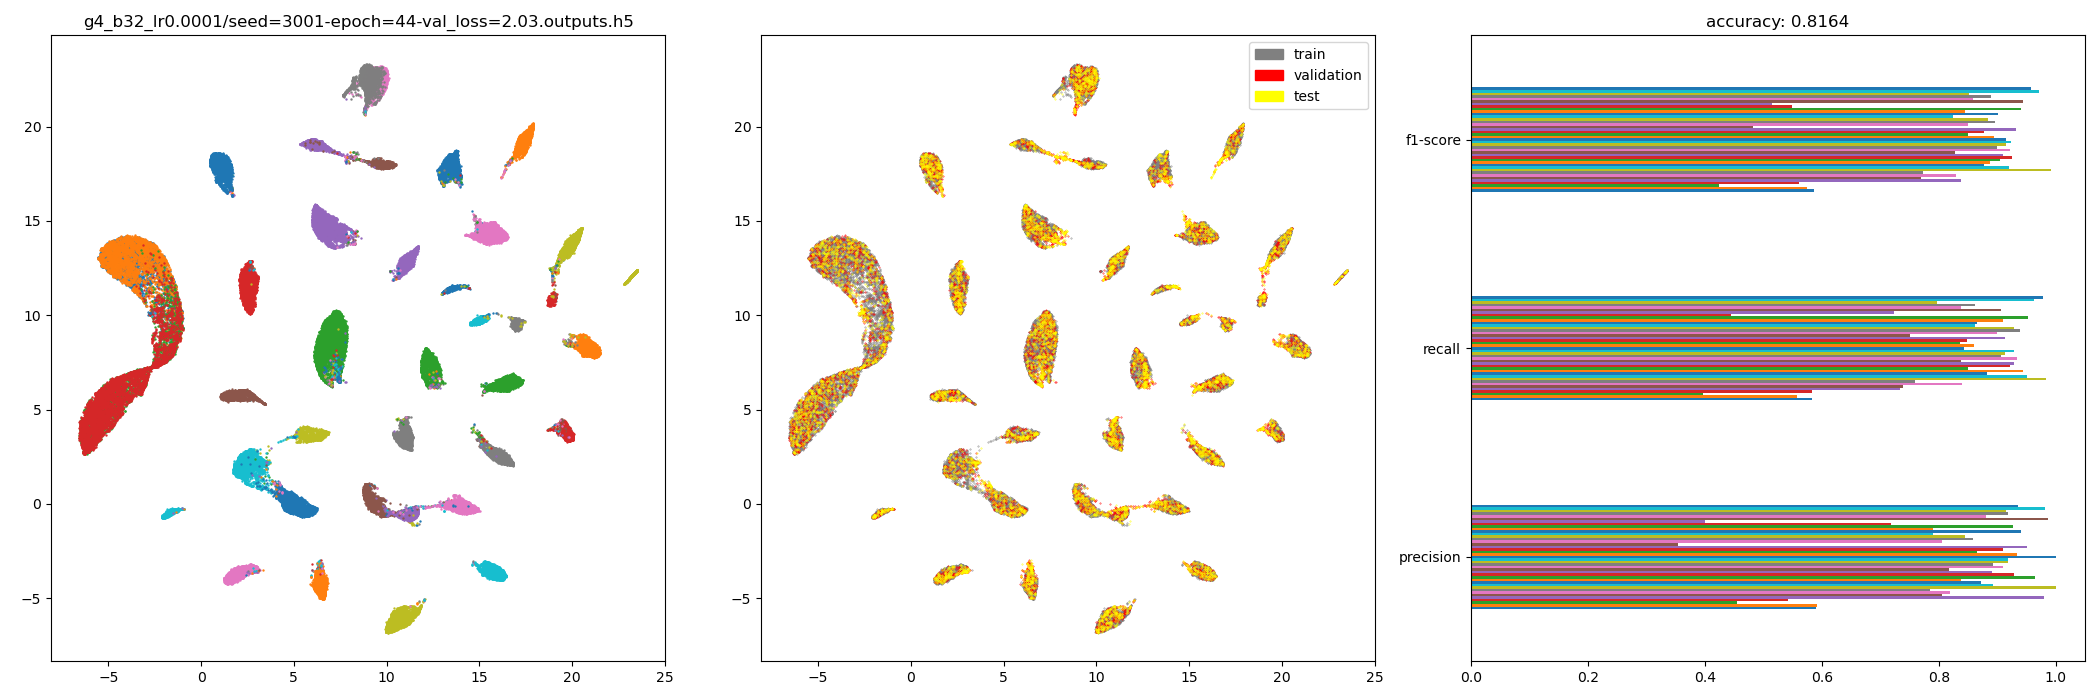
\includegraphics[width=\linewidth]{new_journal/figures/experiments/roznet_multi/4_heads/run3.png}
  \caption{Run 3}
\end{figure}

\begin{figure}[h!]
  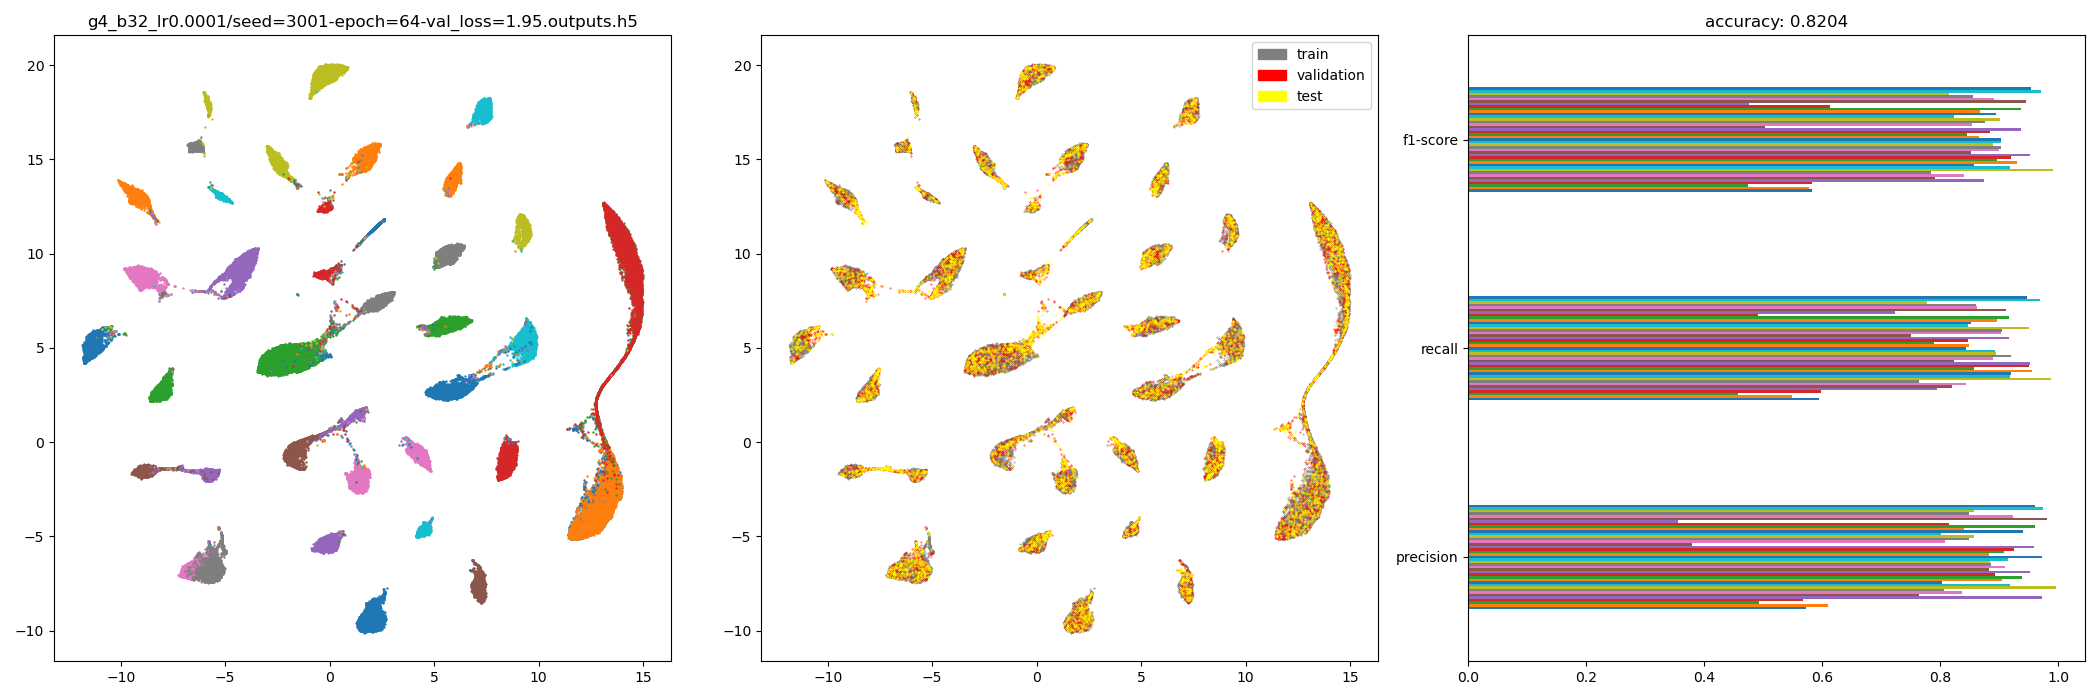
\includegraphics[width=\linewidth]{new_journal/figures/experiments/roznet_multi/4_heads/run4.png}
  \caption{Run 4}
\end{figure}

\vfill
\clearpage

\subsection*{Medium dataset: 8 heads - 80 epochs per run}
Each 4 hour run reached the maximum time limit at 80 epochs. This model did not have as great of a difference in improvement as using 4 heads; however, it does achieve an accuracy of 81.35\% after 4 four runs and is still continuously improving after every run. 

\begin{figure}[h!]
  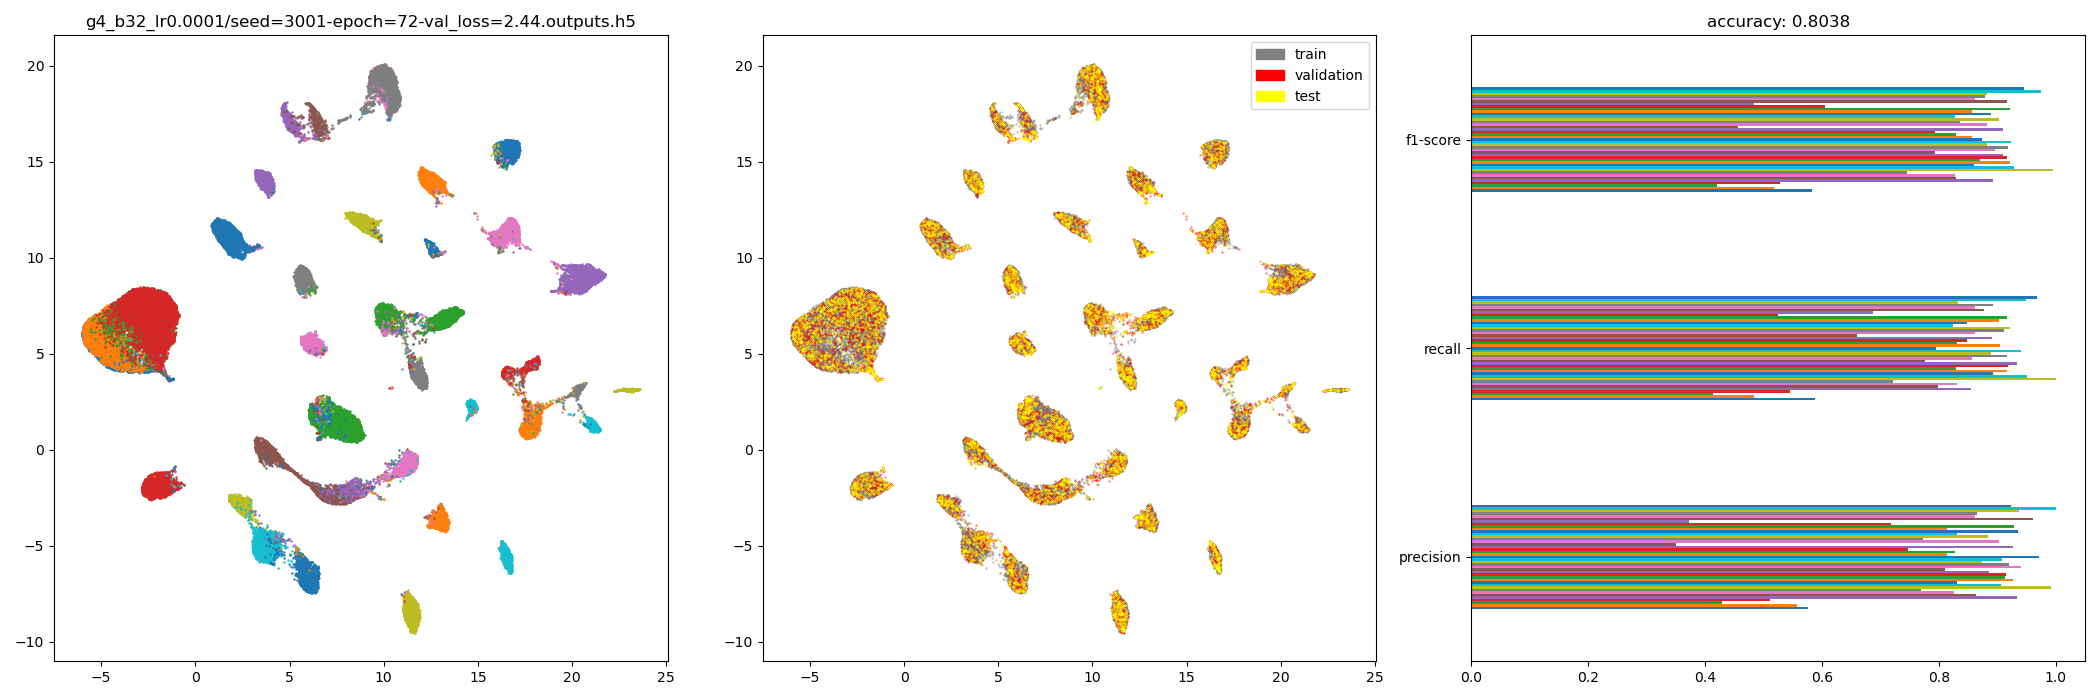
\includegraphics[width=\linewidth]{new_journal/figures/experiments/roznet_multi/8_heads/run1.png}
  \caption{Run 1}
\end{figure}

\begin{figure}[h!]
  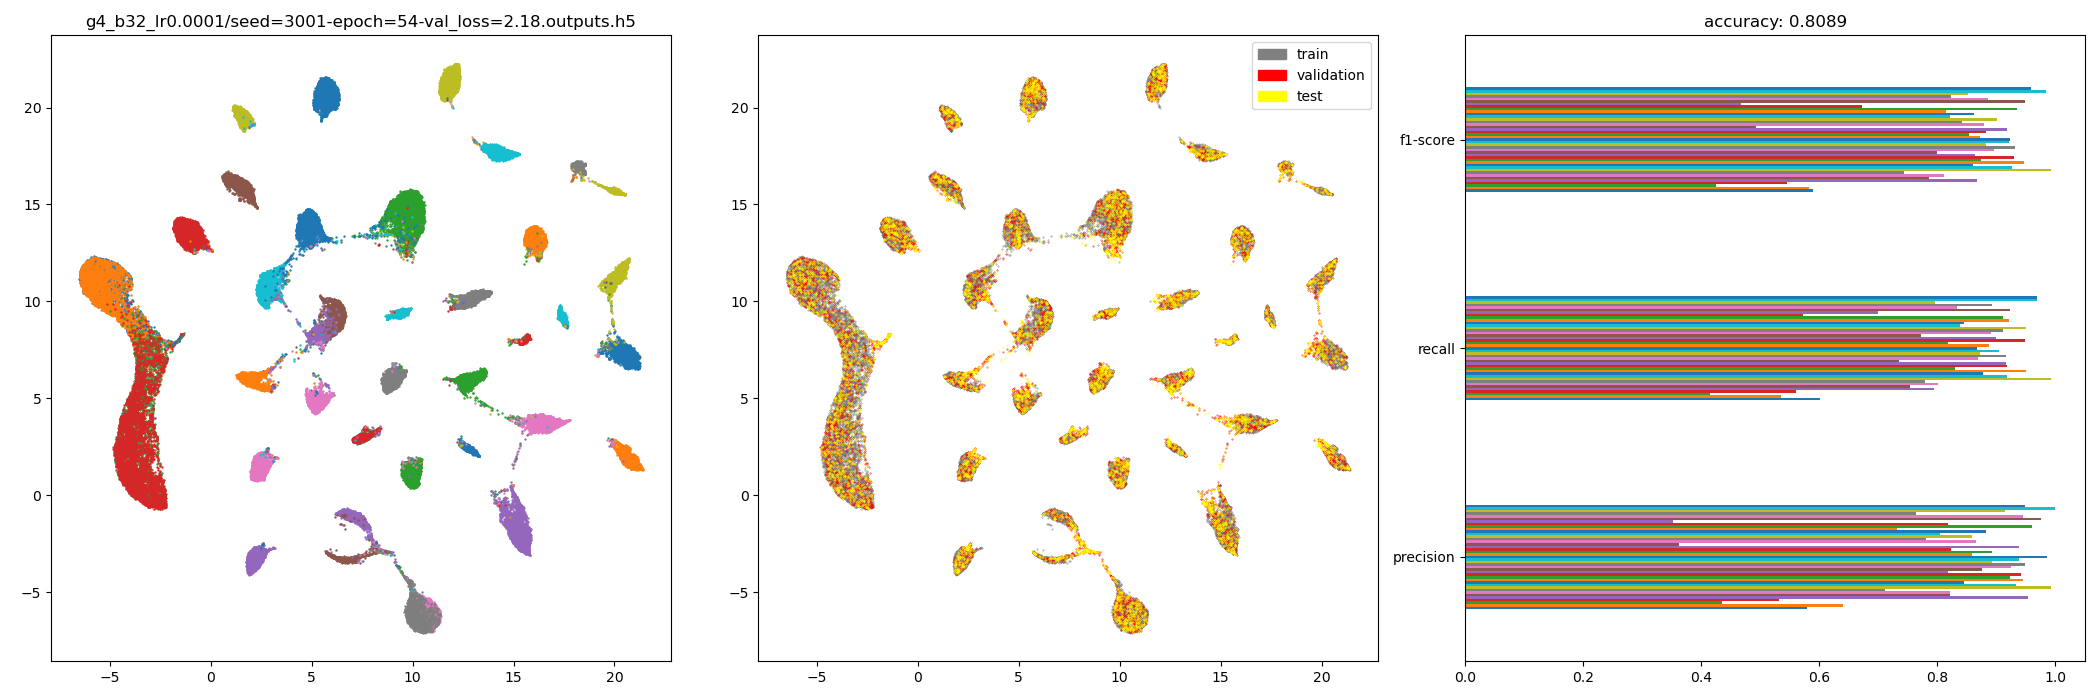
\includegraphics[width=\linewidth]{new_journal/figures/experiments/roznet_multi/8_heads/run2.png}
  \caption{Run 2}
\end{figure}

\begin{figure}[h!]
  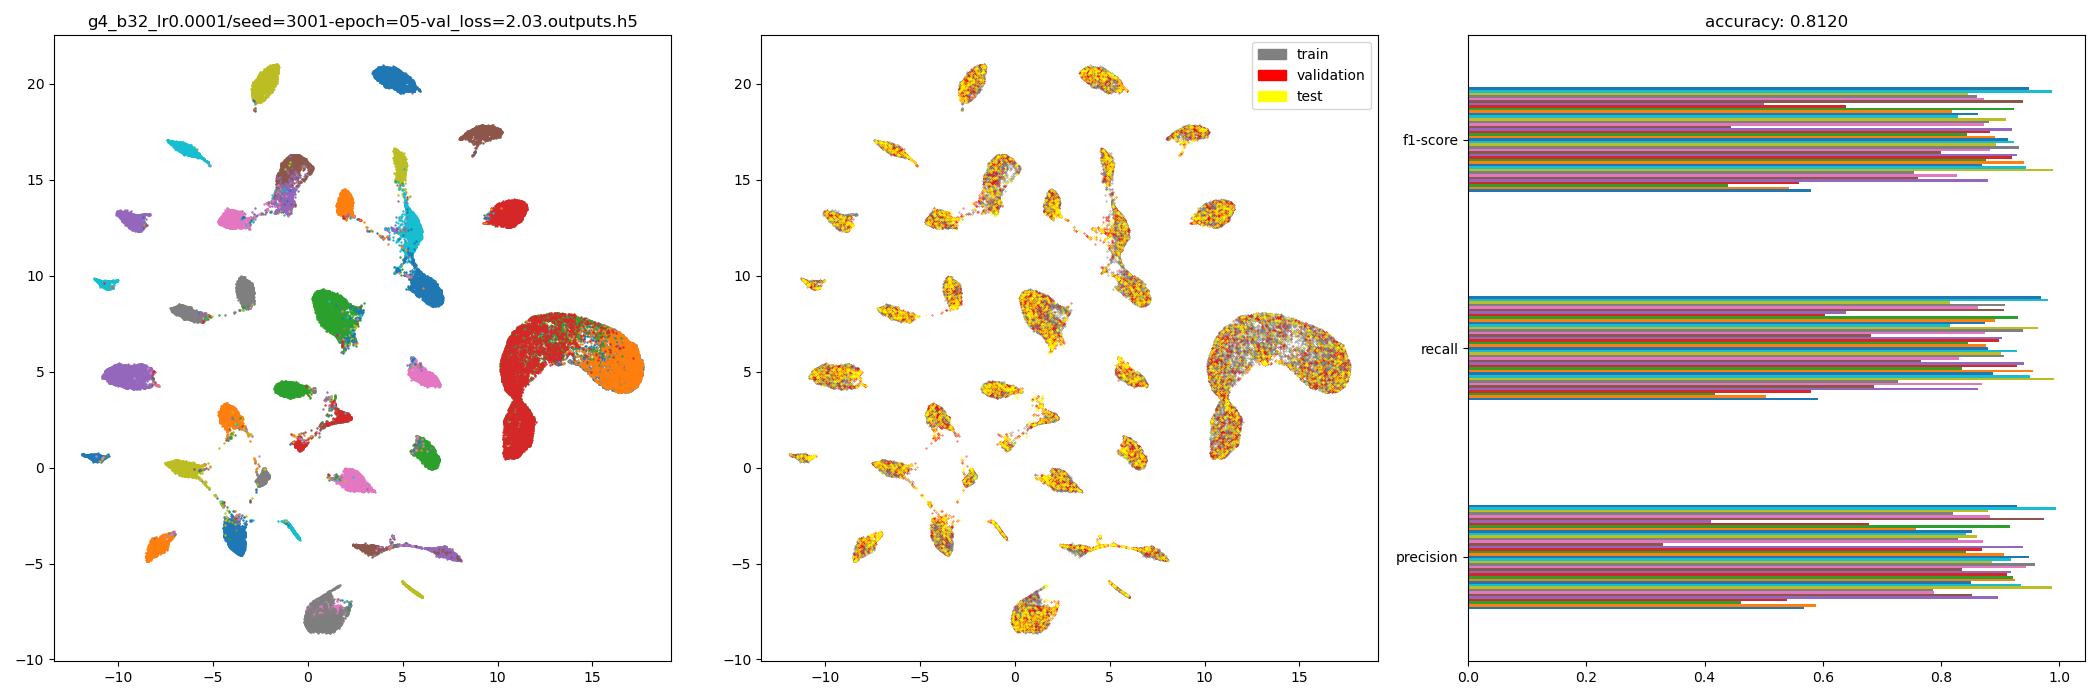
\includegraphics[width=\linewidth]{new_journal/figures/experiments/roznet_multi/8_heads/run3.png}
  \caption{Run 3}
\end{figure}

\begin{figure}[h!]
  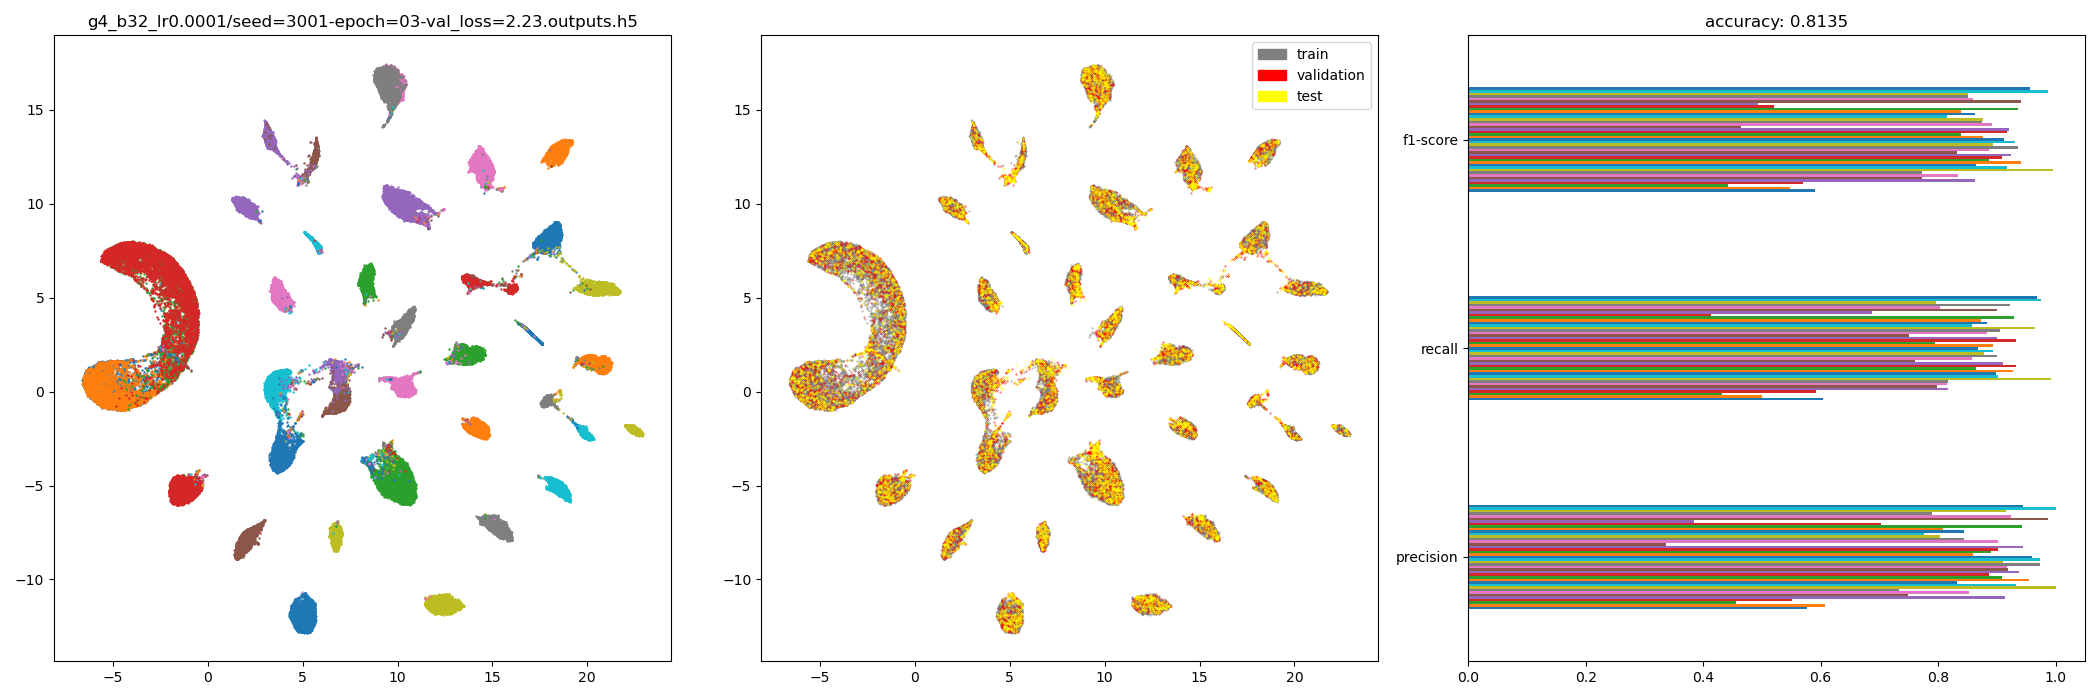
\includegraphics[width=\linewidth]{new_journal/figures/experiments/roznet_multi/8_heads/run4.png}
  \caption{Run 4}
\end{figure}


\clearpage

\subsection*{Medium dataset: 16 heads - 79 epochs per run}
Each 4 hour run reached the maximum time limit at 79 epochs. The best results were achieved at 255/316 epochs with an accuracy of 81.51\%. The accuracy does decreased after the second run. There seems to be more fluctuation in accuracy with more attention heads. 


\begin{figure}[h!]
  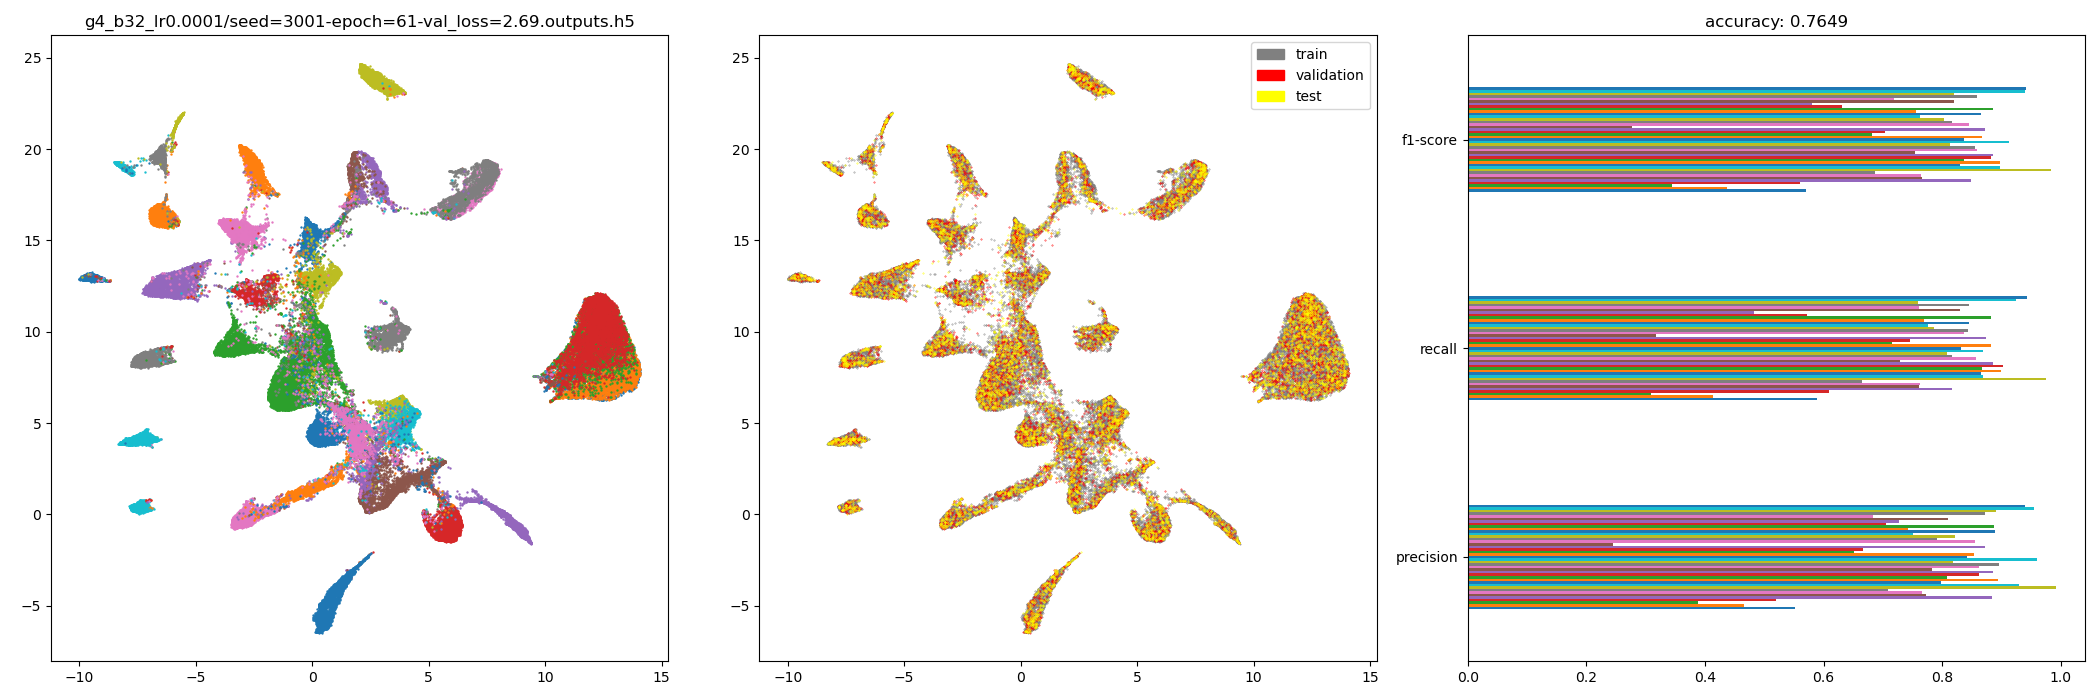
\includegraphics[width=\linewidth]{new_journal/figures/experiments/roznet_multi/16_heads/run1.png}
  \caption{Run 1}
\end{figure}

\begin{figure}[h!]
  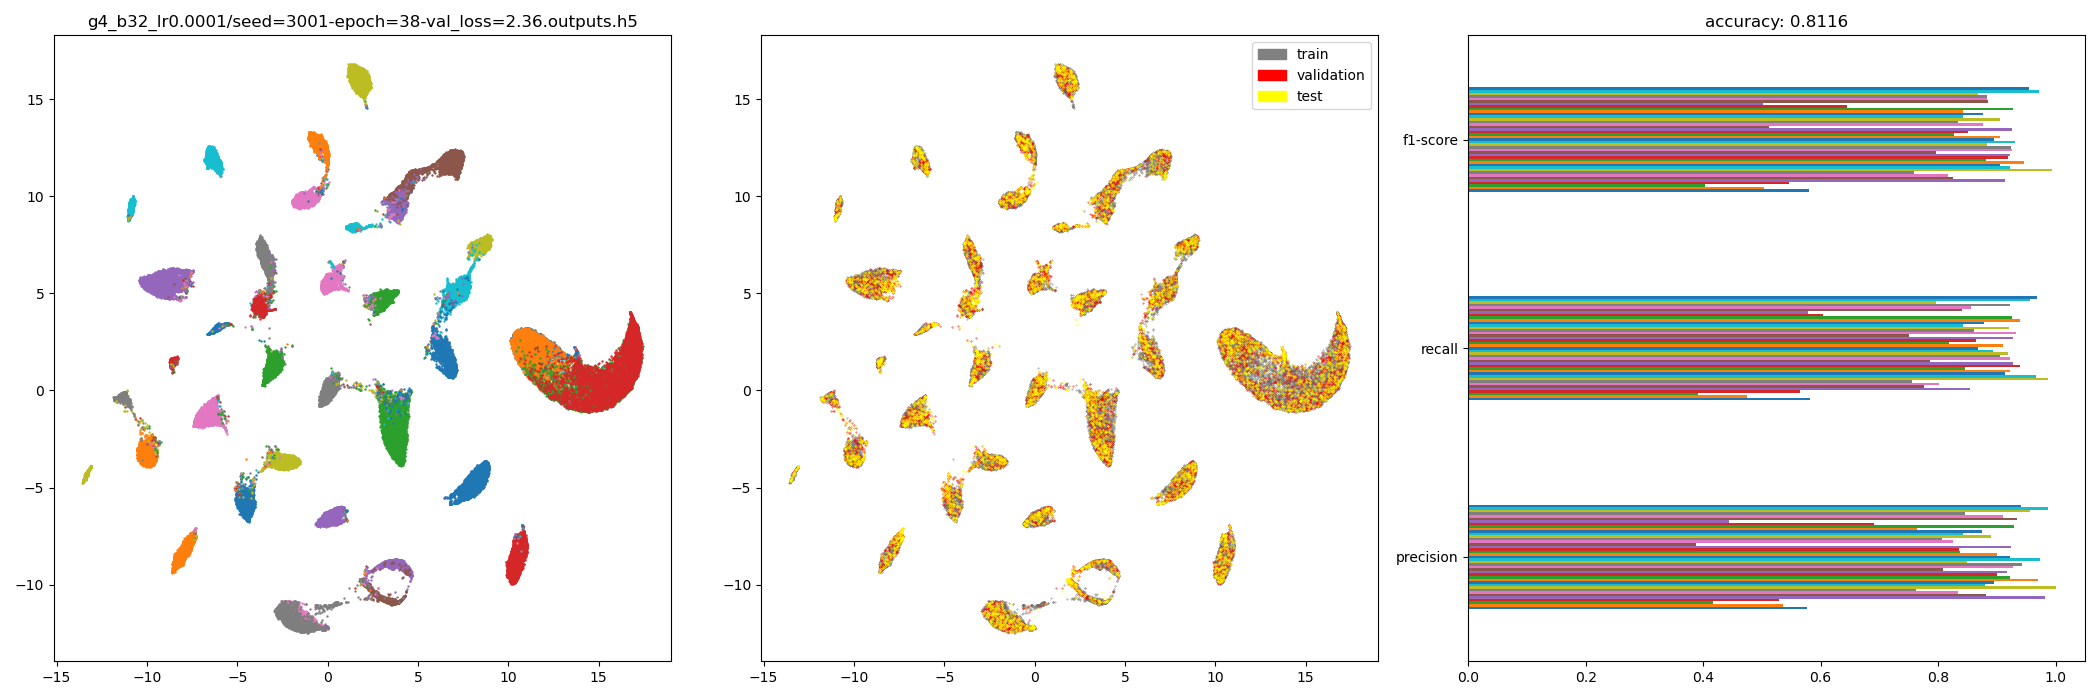
\includegraphics[width=\linewidth]{new_journal/figures/experiments/roznet_multi/16_heads/run2.png}
  \caption{Run 2}
\end{figure}

\begin{figure}[h!]
  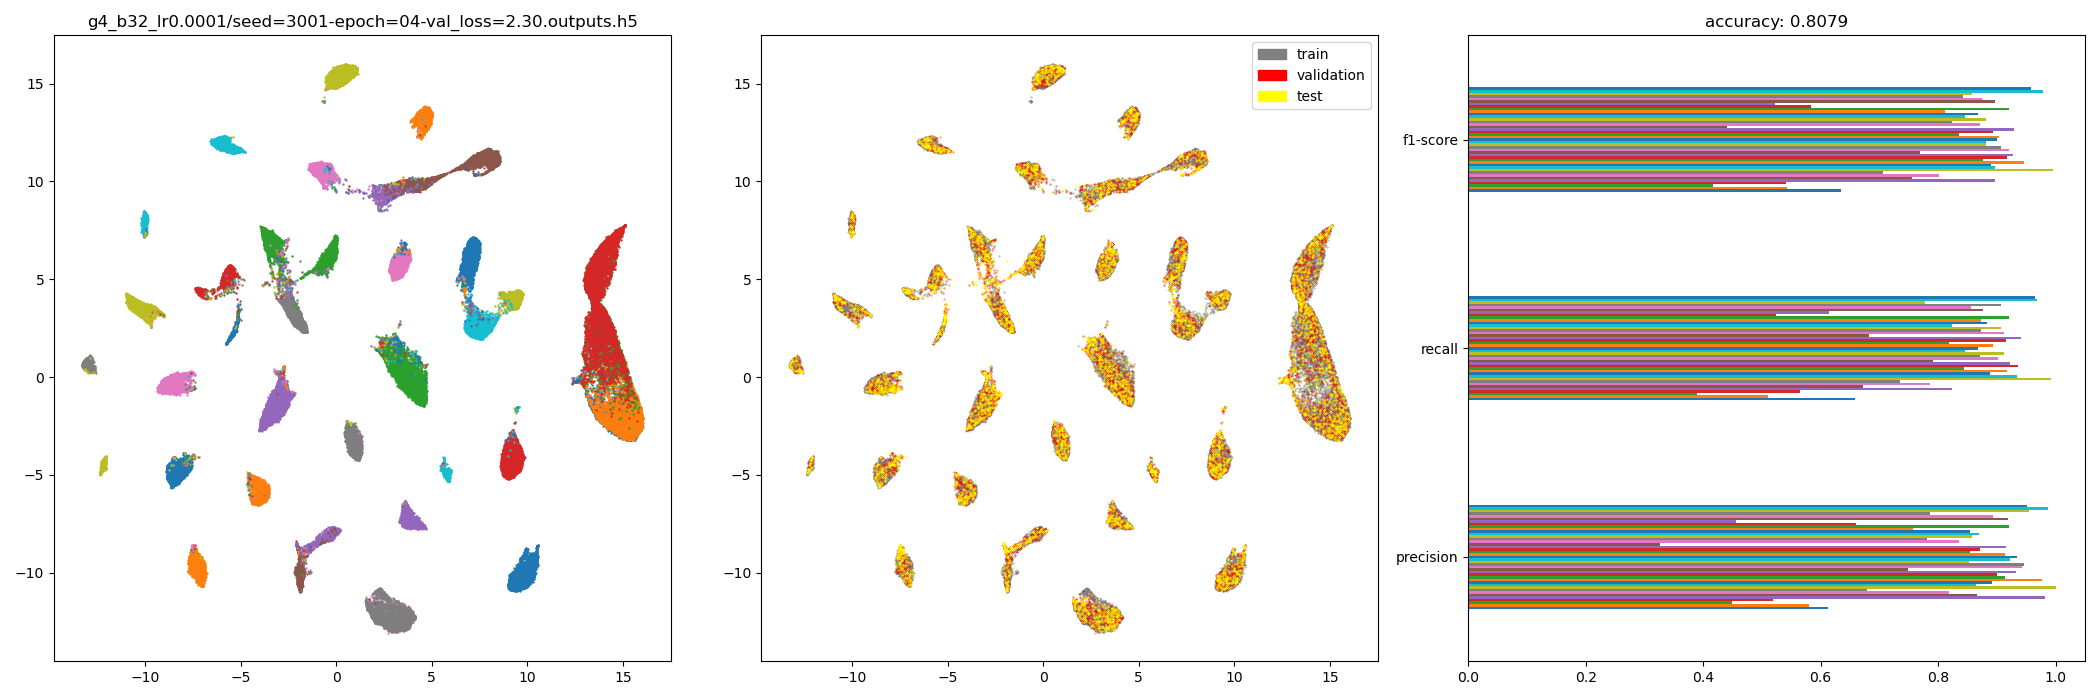
\includegraphics[width=\linewidth]{new_journal/figures/experiments/roznet_multi/16_heads/run3.png}
  \caption{Run 3}
\end{figure}

\begin{figure}[h!]
  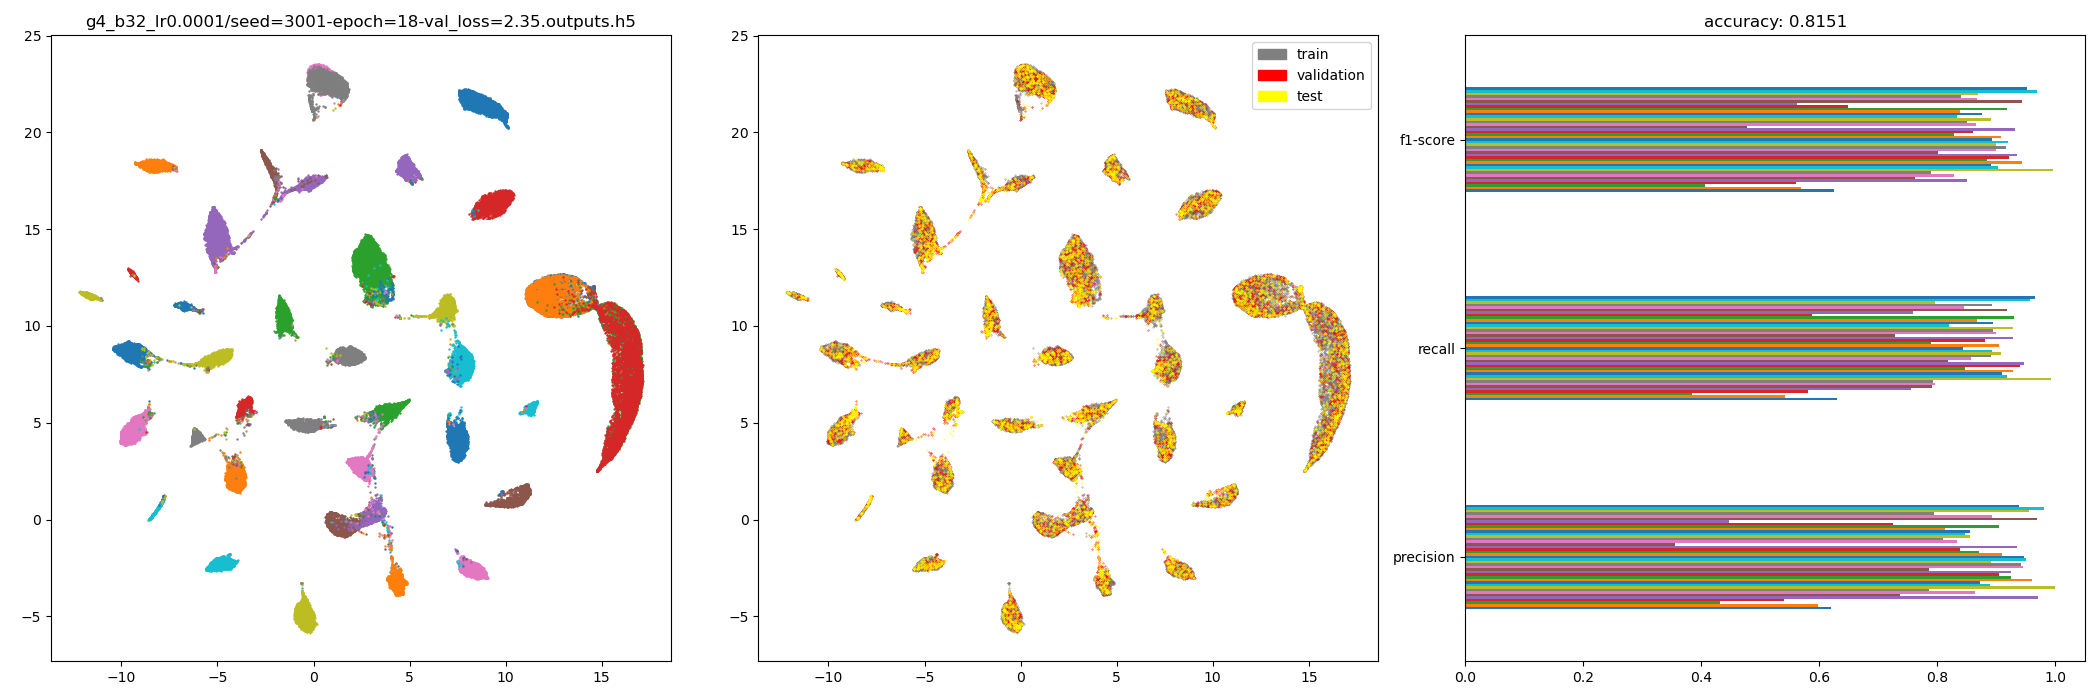
\includegraphics[width=\linewidth]{new_journal/figures/experiments/roznet_multi/16_heads/run4.png}
  \caption{Run 4}
\end{figure}

\clearpage

\subsection*{Medium dataset: -S 2500 -W 2500}
The maximum sequence length and window size that can be used with this model is 2500. Here, Roznet with 8 attention heads was used with -S 2500 -W 2500. This produced similar results as Roznet with 8 attention with -S 1000 -W 1000. 

\begin{figure}[h!]
  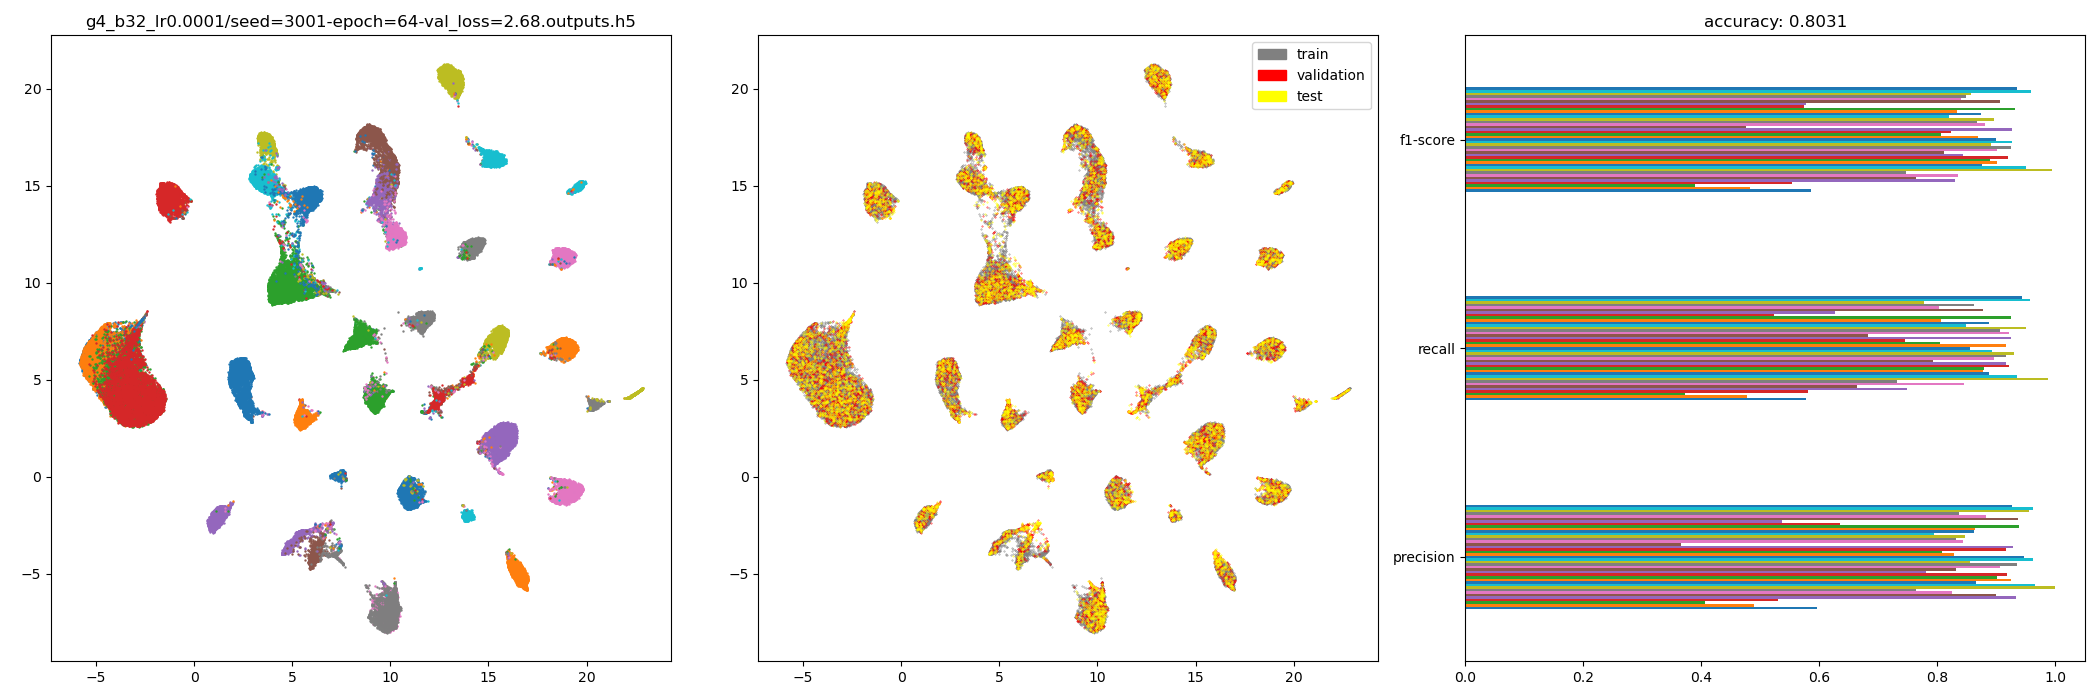
\includegraphics[width=\linewidth]{new_journal/figures/experiments/roznet_multi/S2500_W2500/run1.png}
  \caption{Run 1}
\end{figure}

\begin{figure}[h!]
  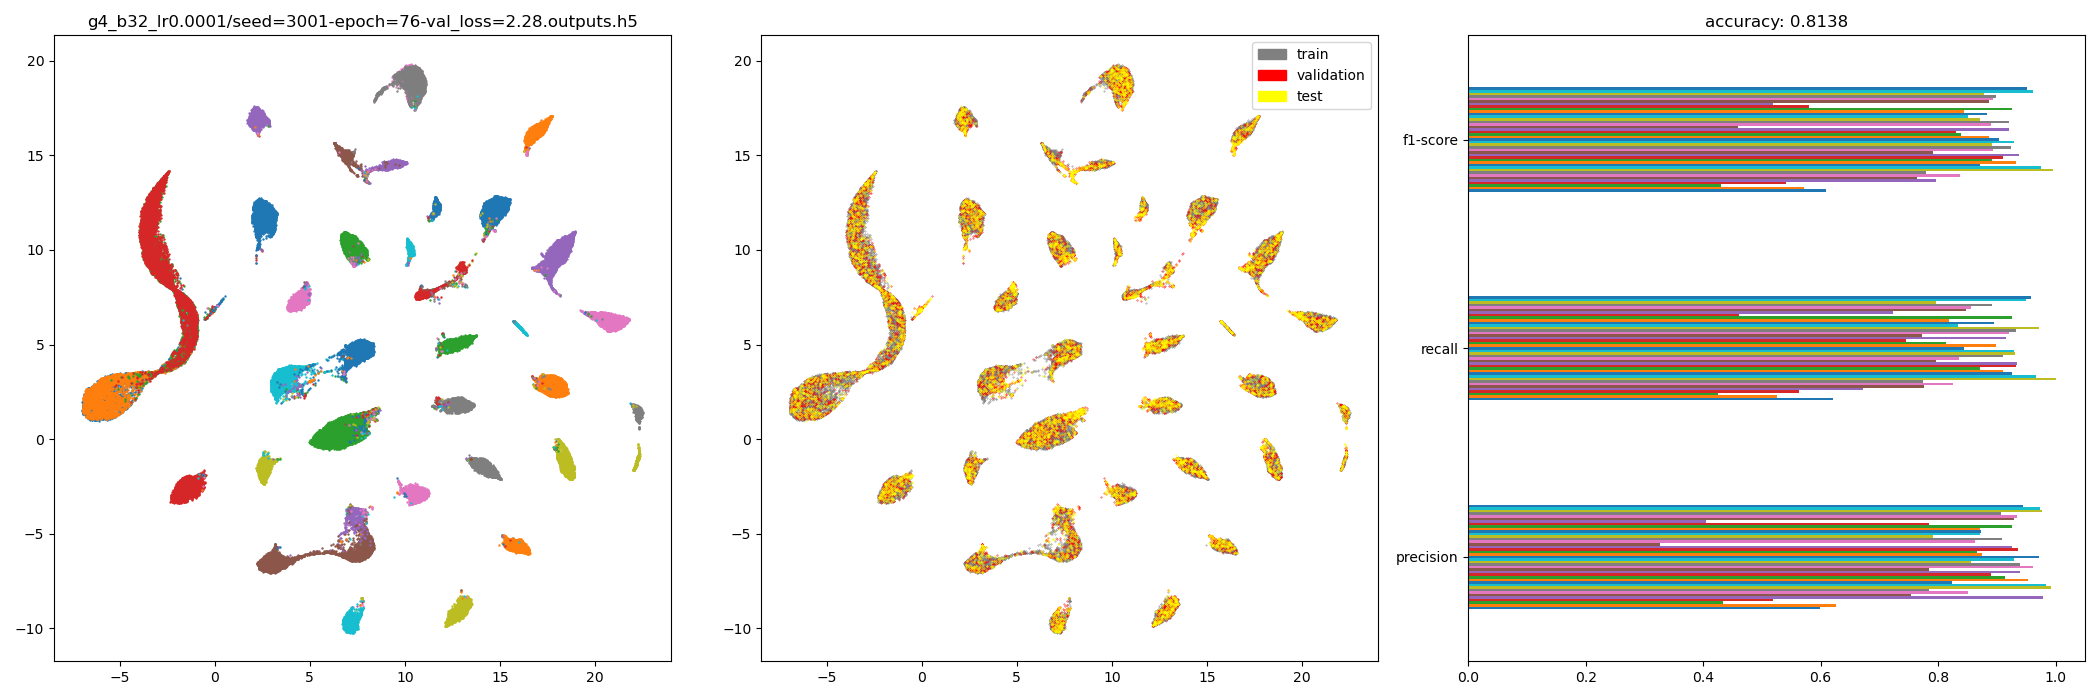
\includegraphics[width=\linewidth]{new_journal/figures/experiments/roznet_multi/S2500_W2500/run2.png}
  \caption{Run 2}
\end{figure}

\begin{figure}[h!]
  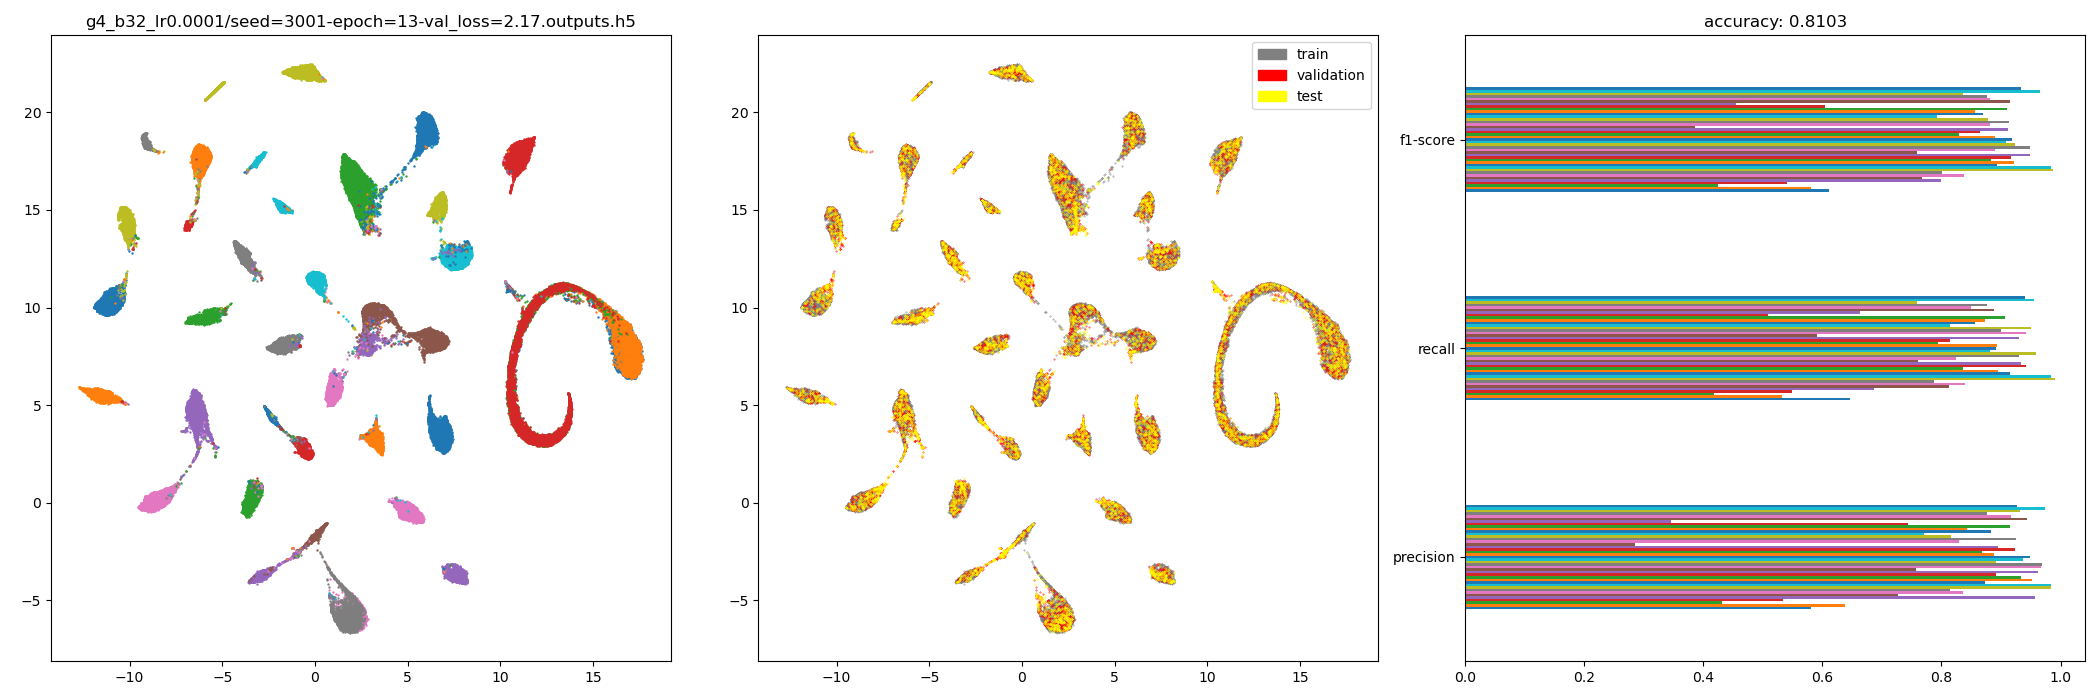
\includegraphics[width=\linewidth]{new_journal/figures/experiments/roznet_multi/S2500_W2500/run3.png}
  \caption{Run 3}
\end{figure}

\end{document}

